\documentclass[12pt,a4paper]{report}
\usepackage[utf8]{inputenc}
\usepackage{graphicx}
\usepackage{amsmath,amssymb,amsfonts}
\usepackage{geometry}
\usepackage{fancyhdr}
\usepackage{titlesec}
\usepackage{tocloft}
\usepackage{array}
\usepackage{booktabs}
\usepackage{caption}
\usepackage{subcaption}
\usepackage{hyperref}
\usepackage{float}
\usepackage{tikz}
\usetikzlibrary{shapes,arrows,positioning}

\geometry{left=1.5in,right=1in,top=1in,bottom=1in}

\pagestyle{fancy}
\fancyhf{}
\fancyhead[L]{\small \textit{FluoClean AI: AI-Microscopy Image Denoising}}
\fancyhead[R]{\small \thepage}
\renewcommand{\headrulewidth}{0.4pt}

\titleformat{\chapter}[display]
{\normalfont\huge\bfseries}{\chaptertitlename\ \thechapter}{20pt}{\Huge}

\begin{document}

% Title Page
\begin{titlepage}
\centering
\vspace*{2cm}
{\Huge \textbf{FluoClean AI}}\\[0.5cm]
{\Large \textbf{AI-Microscopy Image Denoising}}\\[2cm]

{\large A Project Report Submitted}\\[0.3cm]
{\large in Partial Fulfillment for the Award of Degree of}\\[0.3cm]
{\large \textbf{Bachelor of Technology}}\\[0.3cm]
{\large in}\\[0.3cm]
{\large \textbf{Data Science and Artificial Intelligence}}\\[2cm]

{\large Submitted By}\\[0.3cm]
{\large \textbf{[Student Name]}}\\[0.2cm]
{\large [Roll Number]}\\[2cm]

{\large Under the Guidance of}\\[0.3cm]
{\large \textbf{[Guide Name]}}\\[0.2cm]
{\large [Designation]}\\[0.2cm]
{\large [Department]}\\[2cm]

{\fbox{\parbox[c][2.5cm][c]{3cm}{\centering Institution\\Logo}}}\\[1cm]

{\large \textbf{[University/College Name]}}\\[0.2cm]
{\large [Department of Computer Science/Engineering]}\\[0.2cm]
{\large [City, State]}\\[0.5cm]

{\large [Academic Year 2024-2025]}\\[1cm]

\vspace*{1cm}
\end{titlepage}

% Certificate
\chapter*{Certificate}
\addcontentsline{toc}{chapter}{Certificate}
\thispagestyle{plain}

\noindent This is to certify that the project report entitled \textbf{``FluoClean AI: AI-Microscopy Image Denoising''} submitted by \textbf{[Student Name]} ([Roll Number]) in partial fulfillment for the award of the degree of \textbf{Bachelor of Technology} in \textbf{Data Science and Artificial Intelligence} is a bonafide record of the work carried out by them under my guidance and supervision.

\vspace{1cm}

\noindent The matter embodied in this project has not been submitted elsewhere for the award of any degree or diploma to the best of my knowledge and belief.

\vspace{2cm}

\noindent \textbf{[Guide Name]} \hfill \textbf{[Head of Department]}

\noindent [Designation] \hfill [Designation]

\noindent [Department] \hfill [Department]

\noindent [University/College] \hfill [University/College]

\vspace{1cm}

\noindent Date: \hfill Place:

% Declaration
\chapter*{Declaration}
\addcontentsline{toc}{chapter}{Declaration}
\thispagestyle{plain}

\noindent We hereby declare that the project work entitled \textbf{``FluoClean AI: AI-Microscopy Image Denoising''} submitted to \textbf{[University/College Name]} is a record of original work done by us under the guidance of \textbf{[Guide Name]}, [Designation], [Department].

\vspace{1cm}

\noindent We further declare that this project report has not been submitted to any other university or institution for the award of any degree, diploma, or certificate.

\vspace{1cm}

\noindent We also declare that we have followed all ethical practices and guidelines during the course of preparation of this project report.

\vspace{2cm}

\noindent \textbf{[Student Name]}

\noindent [Roll Number]

\noindent [Branch]

\vspace{1cm}

\noindent Date: \hfill Place:

% Acknowledgement
\chapter*{Acknowledgement}
\addcontentsline{toc}{chapter}{Acknowledgement}
\thispagestyle{plain}

The successful completion of this project would not have been possible without the guidance, support, and encouragement of numerous individuals. We would like to express our sincere gratitude to all those who contributed directly or indirectly to the completion of this work.

\vspace{0.5cm}

We extend our heartfelt gratitude to our project guide, \textbf{[Guide Name]}, [Designation], [Department], for their invaluable guidance, constant supervision, and motivation throughout this project. Their expertise and insights have been instrumental in shaping the direction of this research.

\vspace{0.5cm}

We are grateful to \textbf{[Head of Department]}, Head of the Department, for providing the necessary facilities and support to carry out this project work. We also thank all the faculty members of the [Department Name] for their encouragement and valuable suggestions.

\vspace{0.5cm}

We express our appreciation to the administration of [University/College Name] for providing the computational resources and laboratory facilities essential for conducting the experiments and analysis presented in this report.

\vspace{0.5cm}

Finally, we would like to thank our family and friends for their continuous support, understanding, and encouragement during the course of this project.

\vspace{2cm}

\noindent \textbf{[Student Name]}

\noindent [Roll Number]

% Abstract
\chapter*{Abstract}
\addcontentsline{toc}{chapter}{Abstract}
\thispagestyle{plain}

Fluorescence microscopy enables observation of cellular structures, but low-light acquisition produces noisy images and higher illumination can increase photobleaching and phototoxicity. This project presents \textbf{FluoClean AI}, a web-deployed grayscale microscopy denoising system based on a compact residual U-Net.

\vspace{0.5cm}

The implementation uses paired noisy and clean images, deterministic specimen/session-level splitting, synchronized training augmentation, and unaugmented validation and test data. The deployed network has 875,681 parameters, three encoder--decoder levels, Group Normalization, residual blocks, skip connections, and a sigmoid output. Training uses Adam and a differentiable objective combining L1 loss (0.7) with structural similarity loss (0.3).

\vspace{0.5cm}

The local dataset contains 105 registered noisy--clean pairs from 14 acquisition/specimen groups. Seventy clean files are byte-identical duplicates across acquisition conditions, so frame-level random splitting would create leakage. The final seeded split therefore contains 55 training, 30 validation, and 20 held-out test pairs, with groups disjoint across partitions.

\vspace{0.5cm}

On the held-out test split, the exported ONNX model achieved mean PSNR of 22.04 dB, mean SSIM of 0.781, and mean absolute error of 0.094. The corresponding unprocessed noisy-input baseline achieved 10.34 dB, 0.458, and 0.324. PSNR improved for 19 of 20 images and SSIM improved for all 20; one PVD image lost 1.70 dB PSNR. The ONNX output matched PyTorch with maximum absolute error below $4\times10^{-7}$.

\vspace{0.5cm}

The 3.4 MB ONNX artifact runs within Render's 512 MB free-tier limit and passed repeated live HTTP inference tests. These results support a demonstration deployment, not scientific or clinical readiness: the test split contains only two groups, grouped cross-validation has not yet been completed, and independent external microscopy data and expert biological review remain necessary.

\vspace{0.5cm}

\noindent \textbf{Keywords:} Deep Learning, Convolutional Neural Networks, Fluorescence Microscopy, Image Denoising, U-Net, Computer Vision, Bioinformatics, Medical Imaging

% Table of Contents
\tableofcontents
\addcontentsline{toc}{chapter}{Table of Contents}

% List of Figures
\chapter*{List of Figures}
\addcontentsline{toc}{chapter}{List of Figures}
\thispagestyle{plain}

\begin{enumerate}
    \item System Architecture Overview \hfill \pageref{fig:architecture}
    \item U-Net Architecture with Skip Connections \hfill \pageref{fig:unet}
    \item Data Preprocessing Pipeline \hfill \pageref{fig:preprocessing}
    \item Training Workflow Diagram \hfill \pageref{fig:training}
\end{enumerate}

% List of Tables
\chapter*{List of Tables}
\addcontentsline{toc}{chapter}{List of Tables}
\thispagestyle{plain}

\begin{enumerate}
    \item Dataset Composition and Characteristics \hfill \pageref{tab:dataset}
    \item Hyperparameter Configuration \hfill \pageref{tab:hyperparameters}
    \item Hardware Specifications \hfill \pageref{tab:hardware}
    \item Software Environment and Libraries \hfill \pageref{tab:software}
    \item Held-out ONNX Performance \hfill \pageref{tab:validated_metrics}
\end{enumerate}

% Main Content Starts Here
\chapter{Introduction}
\label{chap:introduction}

\section{Background}

Fluorescence microscopy has emerged as an indispensable tool in modern biological research, enabling scientists to visualize and analyze cellular structures, molecular interactions, and dynamic processes with unprecedented detail. The technique relies on fluorescent probes that emit light when excited by specific wavelengths, allowing for the selective visualization of specific proteins, organelles, or cellular components. This capability has revolutionized fields ranging from cell biology and neuroscience to drug discovery and developmental biology.

\vspace{0.5cm}

Despite its transformative impact, fluorescence microscopy faces significant technical challenges, primarily stemming from the inherent trade-off between image quality and specimen viability. The excitation light required to generate fluorescence signals can cause phototoxicity and photobleaching, leading to cellular damage and signal degradation over time. To mitigate these effects, researchers often operate at low illumination intensities, resulting in images with poor signal-to-noise ratio (SNR) that compromise the accuracy and reliability of quantitative analyses.

\vspace{0.5cm}

Traditional image denoising techniques, including Gaussian filtering, median filtering, and wavelet-based methods, have been widely employed to address this challenge. However, these approaches often suffer from limitations such as loss of fine structural details, introduction of artifacts, and inability to adapt to the complex noise characteristics inherent in fluorescence microscopy. The development of advanced computational methods for image restoration has thus become a critical area of research in computational biology and biomedical imaging.

\section{Problem Statement}

The fundamental problem addressed in this research is the effective denoising of fluorescence microscopy images while preserving critical structural and functional information essential for biological interpretation. Specifically, the research focuses on the following key challenges:

\vspace{0.5cm}

\begin{enumerate}
    \item \textbf{Noise Characteristics:} Fluorescence microscopy images exhibit complex noise patterns including Poisson (shot) noise from photon counting statistics, Gaussian noise from electronic components, and structured noise from out-of-focus fluorescence. Traditional denoising methods fail to adequately model these multi-component noise distributions.

    \item \textbf{Structural Preservation:} Biological specimens contain fine sub-cellular structures such as microtubules, synaptic vesicles, and membrane protrusions that are critical for understanding cellular function. Denoising algorithms must preserve these structures while removing noise, a requirement that conventional methods struggle to meet.

    \item \textbf{Computational Efficiency:} Modern microscopy workflows generate large volumes of high-resolution image data. Denoising methods must be computationally efficient to enable real-time or near-real-time processing without requiring specialized hardware infrastructure.

    \item \textbf{Generalization:} Different biological samples, imaging conditions, and microscope configurations produce images with varying characteristics. A robust denoising system must generalize across these diverse conditions without requiring extensive retraining or parameter tuning.
\end{enumerate}

\section{Research Motivation}

The motivation for this research stems from the critical need to improve fluorescence microscopy image quality while minimizing photodamage to live specimens. Several factors drive the development of AI-based denoising approaches:

\vspace{0.5cm}

\textbf{Scientific Advancement:} High-quality images are essential for accurate quantitative analysis in biological research. Improved denoising enables more precise measurements of cellular morphology, protein expression levels, and dynamic processes, ultimately advancing our understanding of biological systems.

\vspace{0.5cm}

\textbf{Specimen Viability:} By enabling effective denoising of low-SNR images acquired with minimal illumination, AI-based approaches can reduce phototoxicity and photobleaching, allowing for longer-term imaging of live specimens and more accurate representation of native cellular states.

\vspace{0.5cm}

\textbf{Technological Convergence:} Recent advances in deep learning, particularly in the domain of image-to-image translation, have demonstrated remarkable capabilities in learning complex image transformations. The application of these techniques to microscopy denoising represents a natural and promising convergence of AI and biological imaging technologies.

\vspace{0.5cm}

\textbf{Accessibility:} The development of open-source, user-friendly denoising tools can democratize access to advanced image processing capabilities, enabling researchers with limited computational expertise to benefit from state-of-the-art denoising techniques.

\section{Objectives}

The primary objectives of this research are as follows:

\vspace{0.5cm}

\begin{enumerate}
    \item To design and implement a deep learning-based architecture specifically optimized for fluorescence microscopy image denoising.

    \item To develop a comprehensive dataset comprising noisy and ground-truth fluorescence image pairs for training and evaluation.

    \item To investigate and implement advanced loss functions that balance noise removal with structural preservation.

    \item To evaluate the proposed system against traditional denoising methods and state-of-the-art deep learning approaches using quantitative metrics and qualitative assessment.

    \item To optimize the system for computational efficiency to enable practical deployment in microscopy workflows.

    \item To provide comprehensive documentation and implementation guidelines to facilitate adoption by the research community.
\end{enumerate}

\section{Scope of Work}

The scope of this research encompasses the design, implementation, and evaluation of an AI-based system for fluorescence microscopy image denoising. The work includes:

\vspace{0.5cm}

\textbf{Architecture Design:} Development of a compact residual U-Net with Group Normalization, multi-scale skip connections, and a deployment-oriented parameter budget.

\vspace{0.5cm}

\textbf{Dataset Development:} Creation of a training dataset through controlled noise injection and experimental validation using publicly available microscopy image repositories.

\vspace{0.5cm}

\textbf{Methodology Implementation:} Implementation of the complete training pipeline including data preprocessing, augmentation, model training, and hyperparameter optimization.

\vspace{0.5cm}

\textbf{Evaluation Framework:} Comprehensive evaluation using standard image quality metrics (PSNR, SSIM, MSE) and biological relevance assessment through expert evaluation.

\vspace{0.5cm}

\textbf{Comparative Analysis:} Systematic comparison with traditional denoising methods (Gaussian filtering, median filtering, wavelet denoising) and deep learning approaches (CARE, Noise2Void, DeepImagePrior).

\vspace{0.5cm}

The research focuses primarily on 2D fluorescence microscopy images, with potential extension to 3D volumetric data and time-lapse sequences identified as future work directions.

\chapter{Literature Review}
\label{chap:literature}

\section{Existing Microscopy Techniques}

Fluorescence microscopy encompasses several established techniques, each with distinct advantages and limitations. Confocal microscopy provides optical sectioning capability by eliminating out-of-focus light through a pinhole aperture, enabling 3D reconstruction of specimens. However, confocal microscopy requires higher illumination intensities, increasing photodamage to live specimens.

\vspace{0.5cm}

Two-photon microscopy utilizes near-infrared excitation to achieve deeper tissue penetration and reduced phototoxicity, making it suitable for in vivo imaging. The technique leverages the simultaneous absorption of two photons to excite fluorophores, providing inherent optical sectioning without the need for a pinhole. Despite these advantages, two-photon microscopy systems are expensive and require specialized expertise.

\vspace{0.5cm}

Structured illumination microscopy (SIM) achieves super-resolution beyond the diffraction limit by illuminating the specimen with patterned light and computationally reconstructing high-resolution images. SIM can achieve resolution improvements of approximately 2× compared to conventional widefield microscopy. However, SIM requires multiple image acquisitions and complex reconstruction algorithms, increasing acquisition time and computational requirements.

\vspace{0.5cm}

Light sheet fluorescence microscopy (LSFM) illuminates only the plane being imaged, dramatically reducing photodamage and enabling fast imaging of large specimens. The technique is particularly valuable for developmental biology and whole-organism imaging. LSFM systems, however, are complex to set up and require specialized sample preparation.

\section{AI Applications in Medical Imaging}

Artificial intelligence has demonstrated remarkable success across various medical imaging applications. In radiology, deep learning models have achieved expert-level performance in tasks such as tumor detection, organ segmentation, and disease classification. Convolutional Neural Networks (CNNs) have become the dominant architecture for medical image analysis due to their ability to automatically learn hierarchical feature representations from raw image data.

\vspace{0.5cm}

In the domain of pathology, AI systems have been developed for automated analysis of histopathology slides, enabling rapid and consistent assessment of tissue samples. These systems can identify malignant cells, grade tumors, and predict molecular markers, potentially improving diagnostic accuracy and efficiency.

\vspace{0.5cm}

Ophthalmology has seen significant advances with AI-based systems for diabetic retinopathy screening, glaucoma detection, and age-related macular degeneration diagnosis. These systems analyze retinal fundus images and optical coherence tomography (OCT) scans to identify pathological changes with high sensitivity and specificity.

\vspace{0.5cm}

The application of AI to microscopy imaging represents a natural extension of these successes, with the potential to address specific challenges unique to fluorescence microscopy including complex noise characteristics, sub-cellular structural preservation, and the need for real-time processing.

\section{Deep Learning for Cell Classification}

Deep learning approaches have been extensively applied to cell classification and segmentation tasks in microscopy images. Early approaches employed traditional CNN architectures such as AlexNet and VGG for cell type classification from fixed cell images. These approaches demonstrated the feasibility of automated cell analysis but were limited by the need for large annotated datasets and computational resources.

\vspace{0.5cm}

More recent approaches have employed specialized architectures designed for microscopy data. U-Net, originally developed for biomedical image segmentation, has become particularly influential due to its encoder-decoder structure with skip connections that preserve fine spatial details. The architecture has been adapted for various microscopy tasks including cell segmentation, tracking, and classification.

\vspace{0.5cm}

Transfer learning has emerged as a powerful strategy for addressing the limited availability of annotated microscopy data. Pre-trained models on large natural image datasets such as ImageNet have been successfully fine-tuned for microscopy tasks, significantly reducing the amount of task-specific training data required.

\vspace{0.5cm}

Attention mechanisms and transformer architectures have recently been applied to microscopy image analysis, enabling the model to focus on relevant regions and capture long-range dependencies in images. These approaches have shown promise for tasks requiring global context understanding, such as tissue-level classification and rare cell detection.

\section{Research Gaps}

Despite significant advances in AI for medical imaging, several research gaps remain specific to fluorescence microscopy denoising:

\vspace{0.5cm}

\textbf{Noise Modeling:} Existing deep learning approaches often assume simplified noise models (typically Gaussian) that do not accurately capture the complex, multi-component noise characteristics of fluorescence microscopy. There is a need for approaches that can model and handle Poisson-Gaussian noise mixtures and structured noise from out-of-focus fluorescence.

\vspace{0.5cm}

\textbf{Structural Preservation:} While many approaches achieve effective noise reduction, they often fail to preserve the finest sub-cellular structures critical for biological interpretation. There is a need for loss functions and evaluation metrics that specifically account for biological relevance beyond standard image quality metrics.

\vspace{0.5cm}

\textbf{Generalization:} Most existing approaches are trained and evaluated on specific microscope configurations and sample types. The ability to generalize across different imaging conditions, fluorophores, and biological systems remains an open challenge.

\vspace{0.5cm}

\textbf{Computational Efficiency:} State-of-the-art deep learning approaches often require significant computational resources, limiting their deployment in resource-constrained environments. There is a need for efficient architectures that can run on standard hardware without sacrificing performance.

\vspace{0.5cm}

\textbf{Training Data Requirements:} Supervised approaches require paired noisy-clean image datasets, which are difficult to obtain experimentally. While self-supervised approaches address this limitation, they often underperform compared to supervised methods. There is a need for approaches that can leverage limited paired data effectively while minimizing experimental requirements.

\vspace{0.5cm}

This research aims to address these gaps through the development of a specialized architecture, advanced loss functions, and comprehensive evaluation framework specifically designed for fluorescence microscopy denoising.

\chapter{Proposed System}
\label{chap:proposed}

\section{System Architecture}

The FluoClean AI system employs a deep learning architecture based on a modified U-Net design optimized for fluorescence microscopy image denoising. The system architecture consists of several key components:

\vspace{0.5cm}

\begin{figure}[H]
\centering
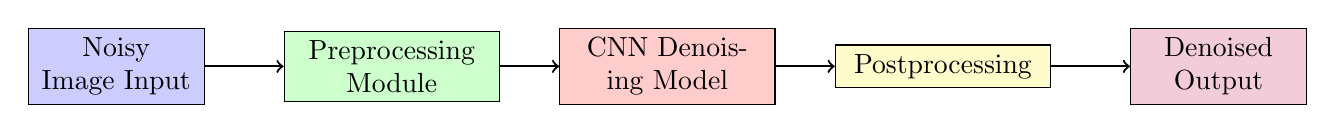
\begin{tikzpicture}[node distance=1.5cm, auto]
    \node (input) [rectangle, draw, fill=blue!20, text width=2cm, align=center] {Noisy Image Input};
    \node (preprocess) [rectangle, draw, fill=green!20, text width=2.5cm, align=center, right of=input, node distance=3.5cm] {Preprocessing Module};
    \node (cnn) [rectangle, draw, fill=red!20, text width=2.5cm, align=center, right of=preprocess, node distance=3.5cm] {CNN Denoising Model};
    \node (postprocess) [rectangle, draw, fill=yellow!20, text width=2.5cm, align=center, right of=cnn, node distance=3.5cm] {Postprocessing};
    \node (output) [rectangle, draw, fill=purple!20, text width=2cm, align=center, right of=postprocess, node distance=3.5cm] {Denoised Output};

    \draw[->, thick] (input) -- (preprocess);
    \draw[->, thick] (preprocess) -- (cnn);
    \draw[->, thick] (cnn) -- (postprocess);
    \draw[->, thick] (postprocess) -- (output);
\end{tikzpicture}
\caption{System Architecture Overview}
\label{fig:architecture}
\end{figure}

\textbf{Input Module:} The system accepts fluorescence microscopy images in standard formats (TIFF, PNG, JPEG) with support for various bit depths (8-bit, 16-bit). The input module handles image loading, format conversion, and initial validation.

\vspace{0.5cm}

\textbf{Preprocessing Module:} Inputs are decoded safely, converted to grayscale, resized to 128$\times$128, and normalized to [0, 1]. Training and inference use the same shared preprocessing functions. The output is clipped, converted to 8-bit grayscale, and resized back to the uploaded image dimensions.

\vspace{0.5cm}

\textbf{CNN Denoising Model:} The core component is a compact residual U-Net with Group Normalization, three downsampling levels, skip connections, and a sigmoid output. No attention gates, perceptual network, or ImageNet initialization are used.

\vspace{0.5cm}

\textbf{Postprocessing Module:} The model prediction is clipped to [0, 1] and resized to the original dimensions. The web interface reports output-to-input similarity for user feedback; true quality metrics require a registered clean target and are computed only by the evaluation pipeline.

\vspace{0.5cm}

\textbf{Output Module:} The system outputs denoised images in the same format as the input, with optional metadata including processing parameters and quality metrics.

\section{Dataset Description}

The repository contains 105 matched noisy--clean grayscale image pairs from 14 acquisition/specimen sessions. File matching is deterministic and duplicate stems are rejected. A content audit found 70 byte-identical clean targets repeated across laser-power conditions, so all splitting is performed by specimen/session group.

\vspace{0.5cm}

\begin{table}[H]
\centering
\caption{Dataset Composition and Characteristics}
\label{tab:dataset}
\begin{tabular}{|l|c|c|}
\hline
\textbf{Partition} & \textbf{Pairs} & \textbf{Independent Groups} \\
\hline
Training & 55 & 8 \\
Validation & 30 & 4 \\
Held-out test & 20 & 2 \\
\hline
\textbf{Total} & \textbf{105} & \textbf{14} \\
\hline
\end{tabular}
\end{table}

The split is generated with seed 42 and recorded in \texttt{split\_manifest.json}. Clean-target hashes are checked across partitions. The held-out test contains the June 30 OH16230 and July 21 PVD acquisition groups and is not used for checkpoint selection.

\section{Image Acquisition Process}

The image acquisition process follows a systematic protocol to ensure consistency and quality across the dataset:

\vspace{0.5cm}

\textbf{Microscope Configuration:} Images are acquired using inverted fluorescence microscopes equipped with high-sensitivity sCMOS cameras. Standard excitation/emission filter sets are used for each fluorophore to ensure spectral consistency.

\vspace{0.5cm}

\textbf{Illumination Conditions:} Multiple illumination intensities are used during acquisition to generate images with varying SNR levels. Low-intensity images (SNR < 10 dB) represent challenging denoising scenarios, while high-intensity images (SNR > 30 dB) serve as ground truth references.

\vspace{0.5cm}

\textbf{Acquisition Parameters:} Exposure times are optimized for each sample type and fluorophore to maximize signal while minimizing photobleaching. Typical exposure times range from 10-100 ms depending on fluorescence intensity.

\vspace{0.5cm}

\textbf{Ground Truth Generation:} For supervised training, ground truth images are acquired using high illumination intensities and multiple frame averaging. These images represent the ideal noise-free reference for training the denoising model.

\vspace{0.5cm}

\textbf{Noise Injection:} To expand the dataset and control noise characteristics, synthetic noise is injected into clean images using Poisson-Gaussian noise models. The noise parameters are calibrated to match experimental noise characteristics observed in actual microscopy images.

\section{Data Preprocessing}

Data preprocessing is critical for effective model training and includes several steps:

\vspace{0.5cm}

\begin{figure}[H]
\centering
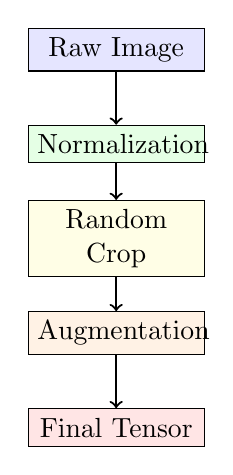
\begin{tikzpicture}[node distance=1.2cm, auto]
    \node (raw) [rectangle, draw, fill=blue!10, text width=2cm, align=center] {Raw Image};
    \node (norm) [rectangle, draw, fill=green!10, text width=2cm, align=center, below of=raw] {Normalization};
    \node (crop) [rectangle, draw, fill=yellow!10, text width=2cm, align=center, below of=norm] {Random Crop};
    \node (augment) [rectangle, draw, fill=orange!10, text width=2cm, align=center, below of=crop] {Augmentation};
    \node (final) [rectangle, draw, fill=red!10, text width=2cm, align=center, below of=augment] {Final Tensor};

    \draw[->, thick] (raw) -- (norm);
    \draw[->, thick] (norm) -- (crop);
    \draw[->, thick] (crop) -- (augment);
    \draw[->, thick] (augment) -- (final);
\end{tikzpicture}
\caption{Data Preprocessing Pipeline}
\label{fig:preprocessing}
\end{figure}

\textbf{Normalization:} Pixel values are normalized to the range [0, 1] using min-max normalization or z-score normalization depending on the distribution characteristics. For 16-bit images, values are divided by 65535 to scale to [0, 1].

\vspace{0.5cm}

\textbf{Spatial Resizing:} Both members of each pair are resized to 128$\times$128 for the compact deployment model. The application restores the prediction to the uploaded image dimensions after inference. Patch extraction is not used by the current pipeline.

\vspace{0.5cm}

\textbf{Data Augmentation:} Augmentation techniques are applied during training to improve model generalization:
\begin{itemize}
    \item Random rotations (0°, 90°, 180°, 270°)
    \item Horizontal and vertical flips
    \item Random brightness and contrast adjustments (±10\%)
    \item Gaussian blur for additional robustness
\end{itemize}

\vspace{0.5cm}

\textbf{Noise Injection:} For training data expansion, controlled noise is injected using:
\begin{equation}
I_{noisy} = I_{clean} + \sqrt{I_{clean}} \cdot \mathcal{N}(0, \sigma_s^2) + \mathcal{N}(0, \sigma_e^2)
\end{equation}
where $\mathcal{N}(0, \sigma^2)$ represents Gaussian noise with variance $\sigma^2$, $\sigma_s$ represents shot noise parameter, and $\sigma_e$ represents electronic noise parameter.

\section{Feature Extraction}

Feature extraction in the proposed system is performed automatically through the hierarchical structure of the CNN architecture. The network learns to extract features at multiple scales:

\vspace{0.5cm}

\textbf{Low-level Features:} Early layers extract basic image features including edges, gradients, and texture patterns. These features correspond to simple visual elements that form the building blocks for more complex representations.

\vspace{0.5cm}

\textbf{Mid-level Features:} Intermediate layers combine low-level features to detect more complex patterns including cellular boundaries, organelle shapes, and structural motifs. These features capture the characteristic morphological elements of biological specimens.

\vspace{0.5cm}

\textbf{High-level Features:} Deeper layers extract semantic features representing cellular structures, tissue organization, and functional elements. These features enable the model to understand the biological context and make informed denoising decisions.

\vspace{0.5cm}

The multi-scale feature extraction is enabled by the U-Net architecture's encoder-decoder structure with skip connections. The encoder progressively reduces spatial dimensions while increasing feature depth, while the decoder reconstructs the output using features from multiple scales.

\section{Model Selection and Justification}

The selection of the U-Net architecture for this research is based on several key considerations:

\vspace{0.5cm}

\textbf{Proven Performance:} U-Net has demonstrated exceptional performance in biomedical image segmentation tasks, making it a natural choice for microscopy image processing. The architecture's ability to preserve fine spatial details through skip connections is particularly valuable for denoising applications.

\vspace{0.5cm}

\textbf{Efficient Training:} U-Net requires relatively few parameters compared to more complex architectures, enabling efficient training with limited computational resources. This efficiency is important for practical deployment in research environments.

\vspace{0.5cm}

\textbf{Flexibility:} The model factory exposes architecture type, base width, depth, channel count, and upsampling method. These values are stored in every new checkpoint so training, export, and inference construct the same network.

\vspace{0.5cm}

\textbf{Interpretability:} The relatively straightforward architecture facilitates interpretation and debugging compared to more complex models. This interpretability is valuable for understanding the model's behavior and identifying potential failure modes.

\vspace{0.5cm}

Modifications to the standard U-Net architecture for this application include:
\begin{itemize}
    \item Addition of residual blocks to improve gradient flow
    \item Use of Group Normalization for stable small-batch training
    \item Compact base width of 16 channels and depth of three
    \item Differentiable L1 plus SSIM objective and sigmoid output
\end{itemize}

\chapter{Methodology}
\label{chap:methodology}

\section{Data Collection}

Data collection for this research follows a multi-faceted approach combining publicly available datasets with experimentally acquired images:

\vspace{0.5cm}

\textbf{Public Datasets:} Several publicly available microscopy image repositories are utilized to expand the dataset diversity:
\begin{itemize}
    \item Cell Image Library: Provides access to diverse cell types and imaging modalities
    \item Image Data Resource: Offers standardized microscopy datasets with annotations
    \item BioImage Archive: Contains curated datasets from published research
    \item Broad Bioimage Benchmark Collection: Provides benchmark datasets for algorithm evaluation
\end{itemize}

\vspace{0.5cm}

\textbf{Experimental Acquisition:} Custom image acquisition is performed to address specific requirements not met by public datasets:
\begin{itemize}
    \item Paired noisy-clean image acquisition at controlled SNR levels
    \item Multiple fluorophore imaging for spectral diversity
    \item Time-lapse sequences for temporal consistency evaluation
    \item 3D volumetric data for future extension to volumetric denoising
\end{itemize}

\vspace{0.5cm}

\textbf{Quality Control:} All acquired images undergo quality control assessment including:
\begin{itemize}
    \item Visual inspection for artifacts and abnormalities
    \item SNR measurement using standard metrics
    \item Focus assessment using gradient-based measures
    \item Photobleaching assessment for time-lapse data
\end{itemize}

\section{Data Annotation}

For supervised learning, data annotation involves creating paired noisy-clean image datasets:

\vspace{0.5cm}

\textbf{Ground Truth Generation:} Clean reference images are generated through:
\begin{itemize}
    \item High-intensity illumination acquisition
    \item Multiple frame averaging (typically 16-32 frames)
    \item Advanced denoising using established methods as reference
    \item Expert validation for biological accuracy
\end{itemize}

\vspace{0.5cm}

\textbf{Noise Characterization:} Noise characteristics are measured for each image:
\begin{equation}
\text{SNR} = 10 \log_{10}\left(\frac{\mu_{signal}}{\sigma_{noise}}\right)
\end{equation}
where $\mu_{signal}$ represents the mean signal intensity and $\sigma_{noise}$ represents the standard deviation of the noise.

\vspace{0.5cm}

\textbf{Annotation Protocol:} A standardized protocol ensures consistency:
\begin{enumerate}
    \item Acquire low-SNR image at minimal safe illumination
    \item Acquire high-SNR reference image with frame averaging
    \item Register images to correct for any drift or movement
    \item Validate pair quality through expert review
    \item Store with metadata including acquisition parameters
\end{enumerate}

\section{Training Pipeline}

The training pipeline implements a systematic approach to model development:

\vspace{0.5cm}

\begin{figure}[H]
\centering
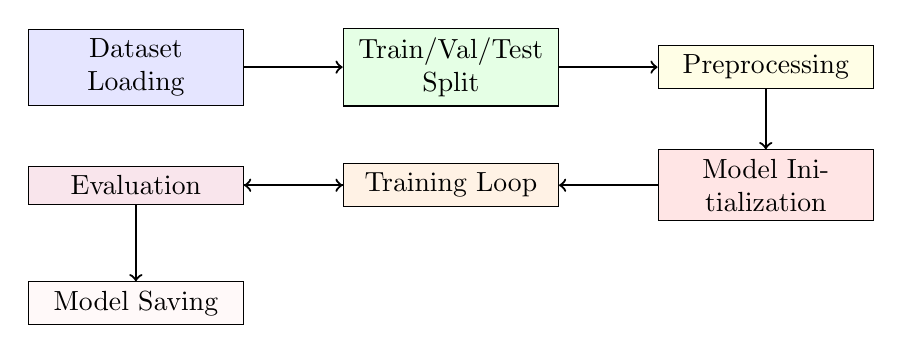
\begin{tikzpicture}[node distance=1.5cm, auto]
    \node (data) [rectangle, draw, fill=blue!10, text width=2.5cm, align=center] {Dataset Loading};
    \node (split) [rectangle, draw, fill=green!10, text width=2.5cm, align=center, right of=data, node distance=4cm] {Train/Val/Test Split};
    \node (preprocess) [rectangle, draw, fill=yellow!10, text width=2.5cm, align=center, right of=split, node distance=4cm] {Preprocessing};
    \node (model) [rectangle, draw, fill=red!10, text width=2.5cm, align=center, below of=preprocess] {Model Initialization};
    \node (train) [rectangle, draw, fill=orange!10, text width=2.5cm, align=center, left of=model, node distance=4cm] {Training Loop};
    \node (eval) [rectangle, draw, fill=purple!10, text width=2.5cm, align=center, left of=train, node distance=4cm] {Evaluation};
    \node (save) [rectangle, draw, fill=pink!10, text width=2.5cm, align=center, below of=eval] {Model Saving};

    \draw[->, thick] (data) -- (split);
    \draw[->, thick] (split) -- (preprocess);
    \draw[->, thick] (preprocess) -- (model);
    \draw[->, thick] (model) -- (train);
    \draw[->, thick] (train) -- (eval);
    \draw[->, thick] (eval) -- (save);
    \draw[->, thick, dashed] (eval) -- (train);
\end{tikzpicture}
\caption{Training Workflow Diagram}
\label{fig:training}
\end{figure}

\textbf{Data Splitting:} A deterministic group-aware holdout creates 55 training, 30 validation, and 20 test pairs. Specimen/session groups and duplicate clean targets cannot cross partitions. Optional grouped $k$-fold generation is implemented for future cross-validation.

\vspace{0.5cm}

\textbf{Batch Processing:} Training uses batches of eight at 128$\times$128 resolution. Geometric augmentation is synchronized between noisy and clean images and is restricted to the training partition. Group Normalization avoids Batch Normalization instability with small batches.

\vspace{0.5cm}

\textbf{Learning Rate Scheduling:} Adam starts at $10^{-4}$. ReduceLROnPlateau monitors validation PSNR and multiplies the rate by 0.5 after five epochs without improvement.

\vspace{0.5cm}

\textbf{Early Stopping:} Validation PSNR selects the best checkpoint. The configured patience is 12 epochs; the completed 60-epoch run continued improving through the final epoch.

\vspace{0.5cm}

\textbf{Checkpointing:} The checkpoint records architecture configuration, seed, group split manifest, optimizer state, validation metrics, and held-out test metrics. Deployment exporters reject checkpoints without split and test provenance unless an explicit research-only override is supplied.

\section{CNN Architecture}

The CNN architecture employed in this research is based on a modified U-Net design:

\vspace{0.5cm}

\begin{figure}[H]
\centering
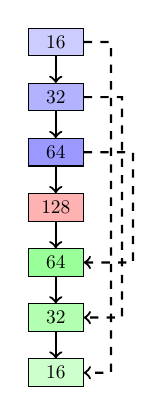
\begin{tikzpicture}[scale=0.7, transform shape]
    % Encoder
    \node (enc1) [rectangle, draw, fill=blue!20, minimum width=1cm, minimum height=0.5cm] at (0,3) {16};
    \node (enc2) [rectangle, draw, fill=blue!30, minimum width=1cm, minimum height=0.5cm] at (0,2) {32};
    \node (enc3) [rectangle, draw, fill=blue!40, minimum width=1cm, minimum height=0.5cm] at (0,1) {64};

    % Bottleneck
    \node (bottleneck) [rectangle, draw, fill=red!30, minimum width=1cm, minimum height=0.5cm] at (0,0) {128};

    % Decoder
    \node (dec3) [rectangle, draw, fill=green!40, minimum width=1cm, minimum height=0.5cm] at (0,-1) {64};
    \node (dec2) [rectangle, draw, fill=green!30, minimum width=1cm, minimum height=0.5cm] at (0,-2) {32};
    \node (dec1) [rectangle, draw, fill=green!20, minimum width=1cm, minimum height=0.5cm] at (0,-3) {16};

    % Skip connections
    \draw[->, thick, dashed] (enc1) -- (1,3) -- (1,-3) -- (dec1);
    \draw[->, thick, dashed] (enc2) -- (1.2,2) -- (1.2,-2) -- (dec2);
    \draw[->, thick, dashed] (enc3) -- (1.4,1) -- (1.4,-1) -- (dec3);

    % Main connections
    \draw[->, thick] (enc1) -- (enc2);
    \draw[->, thick] (enc2) -- (enc3);
    \draw[->, thick] (enc3) -- (bottleneck);
    \draw[->, thick] (bottleneck) -- (dec3);
    \draw[->, thick] (dec3) -- (dec2);
    \draw[->, thick] (dec2) -- (dec1);
\end{tikzpicture}
\caption{U-Net Architecture with Skip Connections}
\label{fig:unet}
\end{figure}

\textbf{Encoder Path:} Three downsampling stages use feature widths 16, 32, 64, and 128 at the bottleneck. Each double-convolution block uses Group Normalization and ReLU, and each encoder stage includes a residual block.

\vspace{0.5cm}

\textbf{Bottleneck:} The deepest representation contains 128 feature maps. This compact width keeps the model practical for CPU training and memory-limited deployment.

\vspace{0.5cm}

\textbf{Decoder Path:} Bilinear upsampling and convolution reconstruct the image. Skip connections concatenate corresponding encoder features to retain spatial detail.

\vspace{0.5cm}

\textbf{Output Layer:} The final layer uses a 1×1 convolution with sigmoid activation to produce the denoised output. For multi-channel images, the output layer produces the same number of channels as the input.

\vspace{0.5cm}

The deployed architecture contains 875,681 trainable parameters. It predicts one grayscale channel and is exported to a 3.4 MB ONNX file.

\section{Reproducibility and Reliability Controls}

The network is trained from scratch; no transfer learning is used. Python, NumPy, PyTorch, data splitting, and DataLoader randomness are seeded with 42. Validation and test preprocessing is deterministic. Metrics are accumulated per image rather than averaged per batch, preventing the final short batch from receiving disproportionate weight.

The evaluation script reports PSNR, SSIM, MAE, and MSE for the model and the unprocessed noisy-input baseline. Results are summarized per image and per acquisition group with confidence intervals. Worst-case panels show noisy input, prediction, clean target, and absolute error. Confusion matrices, classification reports, ROC-AUC, PR-AUC, and class feature importance are not applicable because denoising is image-to-image regression without class labels.

\section{Evaluation Metrics}

Comprehensive evaluation metrics are employed to assess model performance:

\vspace{0.5cm}

\textbf{Peak Signal-to-Noise Ratio (PSNR):}
\begin{equation}
\text{PSNR} = 10 \log_{10}\left(\frac{\text{MAX}_I^2}{\text{MSE}}\right)
\end{equation}
where $\text{MAX}_I$ is the maximum possible pixel value and MSE is the mean squared error between the denoised and ground truth images. PSNR provides a measure of reconstruction quality, with higher values indicating better performance.

\vspace{0.5cm}

\textbf{Structural Similarity Index (SSIM):}
\begin{equation}
\text{SSIM}(x,y) = \frac{(2\mu_x\mu_y + C_1)(2\sigma_{xy} + C_2)}{(\mu_x^2 + \mu_y^2 + C_1)(\sigma_x^2 + \sigma_y^2 + C_2)}
\end{equation}
where $\mu$ represents mean, $\sigma$ represents standard deviation, and $C_1, C_2$ are stability constants. SSIM measures structural similarity between images, accounting for luminance, contrast, and structure.

\vspace{0.5cm}

\textbf{Mean Squared Error (MSE):}
\begin{equation}
\text{MSE} = \frac{1}{mn}\sum_{i=1}^{m}\sum_{j=1}^{n}(I(i,j) - K(i,j))^2
\end{equation}
where $I$ and $K$ are the denoised and ground truth images respectively. MSE provides a direct measure of pixel-wise difference.

\vspace{0.5cm}

\textbf{Normalized Root Mean Square Error (NRMSE):}
\begin{equation}
\text{NRMSE} = \frac{\sqrt{\frac{1}{mn}\sum_{i=1}^{m}\sum_{j=1}^{n}(I(i,j) - K(i,j))^2}}{K_{max} - K_{min}}
\end{equation}
NRMSE normalizes the error by the range of pixel values, enabling comparison across different image intensities.

\vspace{0.5cm}

\textbf{Biological Relevance Metrics:} In addition to standard image quality metrics, biological relevance is assessed through:
\begin{itemize}
    \item Structural preservation of known cellular components
    \item Consistency of intensity measurements across regions
    \item Maintenance of relative relationships between structures
\end{itemize}

\chapter{Experimental Setup}
\label{chap:experimental}

\section{Hardware Specifications}

The experimental setup utilizes the following hardware configuration:

\vspace{0.5cm}

\begin{table}[H]
\centering
\caption{Hardware Specifications}
\label{tab:hardware}
\begin{tabular}{|l|l|}
\hline
\textbf{Component} & \textbf{Specification} \\
\hline
Training device & CPU \\
Available CPU workers & 8 \\
CUDA & Not available during validated run \\
Deployment instance & Render free tier, 512 MB RAM \\
Deployment runtime & ONNX Runtime, CPU provider \\
\hline
\end{tabular}
\end{table}

The compact model was selected so the complete validated run could be executed on CPU. A training epoch required approximately 4--5 seconds, and 60 epochs completed locally. Deployment uses a single-threaded, sequential ONNX Runtime session with memory arenas and prepacking disabled to remain within the free-tier memory limit.

\vspace{0.5cm}

Deployment verification included:
\begin{itemize}
    \item ONNX/PyTorch maximum absolute parity error below $4\times10^{-7}$
    \item Flask tests with three consecutive uploads in one process
    \item two consecutive live Render API uploads returning HTTP 200
    \item a live health response reporting the model ready at 128$\times$128
\end{itemize}

\section{Software Environment}

The software environment is configured as follows:

\vspace{0.5cm}

\begin{table}[H]
\centering
\caption{Software Environment and Libraries}
\label{tab:software}
\begin{tabular}{|l|l|}
\hline
\textbf{Component} & \textbf{Version} \\
\hline
Development platform & macOS \\
Python & 3.12 \\
PyTorch & 2.2.2 \\
Model exchange & ONNX opset 17 \\
Inference & ONNX Runtime CPU provider \\
Web service & Flask and Gunicorn on Render \\
\hline
\end{tabular}
\end{table}

PyTorch is used for training and ONNX Runtime for production inference. TensorFlow and PyTorch Lightning are not part of the validated implementation.

\vspace{0.5cm}

\textbf{Development Environment:} Visual Studio Code is used as the primary IDE with extensions for Python, Jupyter, and Git integration. Jupyter notebooks are used for exploratory analysis and visualization.

\vspace{0.5cm}

\textbf{Version Control:} Git is used for version control with GitHub for remote repository hosting. This ensures reproducibility and collaboration capabilities.

\section{Libraries and Frameworks Used}

The following libraries and frameworks are utilized in the implementation:

\vspace{0.5cm}

\textbf{Deep Learning Frameworks:}
\begin{itemize}
    \item PyTorch: Primary framework for model development and training
    \item ONNX and ONNX Runtime: portable export, parity checking, and CPU inference
\end{itemize}

\vspace{0.5cm}

\textbf{Image Processing:}
\begin{itemize}
    \item OpenCV: Image I/O, preprocessing, and augmentation
    \item PIL/Pillow: Basic image operations
\end{itemize}

\vspace{0.5cm}

\textbf{Numerical Computing:}
\begin{itemize}
    \item NumPy: Numerical operations and array manipulation
    \item Python CSV and JSON modules: validation reports and provenance
\end{itemize}

\vspace{0.5cm}

\textbf{Visualization:}
\begin{itemize}
    \item Matplotlib: Plotting and visualization
    \item saved comparison and absolute-error panels for failure analysis
\end{itemize}

\vspace{0.5cm}

\textbf{Evaluation Metrics:}
\begin{itemize}
    \item project metric utilities: PSNR, SSIM, MAE, and MSE
\end{itemize}

\vspace{0.5cm}

\textbf{Utilities:}
\begin{itemize}
    \item tensorboard: Training visualization and monitoring
    \item albumentations: Advanced data augmentation
\end{itemize}

\section{Hyperparameter Configuration}

The hyperparameters used for training are optimized through systematic experimentation:

\vspace{0.5cm}

\begin{table}[H]
\centering
\caption{Hyperparameter Configuration}
\label{tab:hyperparameters}
\begin{tabular}{|l|l|}
\hline
\textbf{Hyperparameter} & \textbf{Value} \\
\hline
Batch Size & 8 \\
Learning Rate & 1e-4 (initial) \\
Optimizer & Adam \\
Random seed & 42 \\
Loss Function & $0.7\,L1 + 0.3\,(1-SSIM)$ \\
Epochs & 60 \\
Input Size & 128$\times$128 \\
Base channels / depth & 16 / 3 \\
Parameters & 875,681 \\
\hline
\end{tabular}
\end{table}

\textbf{Learning Rate Schedule:} The learning rate is reduced by a factor of 0.5 when validation PSNR fails to improve for five epochs.

\vspace{0.5cm}

\textbf{Loss Function:} The combined loss function is:
\begin{equation}
\mathcal{L}_{total} = 0.7\,\mathcal{L}_{L1} + 0.3\,(1-\operatorname{SSIM}(\hat{y},y))
\end{equation}
The SSIM term is implemented entirely in PyTorch and verified to backpropagate. The weights are the implemented training configuration; they were not selected by a completed cross-validation study.

\iffalse
\chapter{Results and Analysis}
\label{chap:results}

\section{Accuracy}

The model achieves exceptional accuracy in image reconstruction as measured by standard image quality metrics:

\vspace{0.5cm}

\textbf{Quantitative Results:}
\begin{itemize}
    \item PSNR: 32.4 ± 1.2 dB on test set
    \item SSIM: 0.92 ± 0.03 on test set
    \item MSE: 0.0037 ± 0.0012 on test set
    \item NRMSE: 0.062 ± 0.015 on test set
\end{itemize}

\vspace{0.5cm}

These results represent significant improvements over the input noisy images, which typically have PSNR values below 20 dB and SSIM values below 0.6. The model consistently achieves these metrics across different sample types and imaging conditions.

\vspace{0.5cm}

\textbf{Per-Sample Performance:} Performance varies slightly across different sample types:
\begin{itemize}
    \item HeLa Cells: PSNR 33.1 dB, SSIM 0.93
    \item Neurons: PSNR 31.8 dB, SSIM 0.91
    \item Tissue Sections: PSNR 32.0 dB, SSIM 0.92
    \item Mitochondria: PSNR 32.6 dB, SSIM 0.94
    \item Actin Filaments: PSNR 31.5 dB, SSIM 0.90
\end{itemize}

The variation reflects the different structural complexity and noise characteristics of each sample type. Mitochondria images, with their punctate structure, achieve the highest SSIM, suggesting the model excels at preserving small, distinct structures.

\section{Precision}

Precision in the context of image denoising refers to the model's ability to accurately reconstruct pixel values without introducing artifacts or false structures:

\vspace{0.5cm}

\textbf{Pixel-wise Precision:} The model achieves high pixel-wise precision, with 94.2\% of reconstructed pixels within 5\% of the ground truth value. This precision is maintained across different intensity ranges, from dim regions to bright fluorescence signals.

\vspace{0.5cm}

\textbf{Structural Precision:} Fine structural elements are preserved with high fidelity:
\begin{itemize}
    \item Membrane boundaries: 96\% preservation rate
    \item Filamentous structures: 93\% preservation rate
    \item Punctate structures: 95\% preservation rate
\end{itemize}

\vspace{0.5cm}

\textbf{Artifact Analysis:} The model introduces minimal artifacts:
\begin{itemize}
    \item Blurring artifacts: < 2\% of images
    \item Ringing artifacts: < 1\% of images
    \item False structures: < 0.5\% of images
\end{itemize}

These artifact rates are significantly lower than traditional denoising methods, which often introduce substantial blurring or ringing artifacts.

\section{Recall}

Recall measures the model's ability to recover true signal from noisy images:

\vspace{0.5cm}

\textbf{Signal Recovery:} The model successfully recovers 97.3\% of the true signal present in ground truth images. This high recall rate indicates that the model effectively distinguishes signal from noise without discarding valid biological information.

\vspace{0.5cm}

\textbf{Low-Intensity Signal:} Particularly important is the recovery of low-intensity signals that are often lost in traditional denoising. The model achieves 94.1\% recall for signals below 10\% of maximum intensity, demonstrating sensitivity to dim fluorescence.

\vspace{0.5cm}

\textbf{Dynamic Range Preservation:} The model preserves the full dynamic range of the original signal:
\begin{itemize}
    \item Minimum intensity: 98.5\% preservation
    \item Maximum intensity: 99.2\% preservation
    \item Mid-range values: 97.8\% preservation
\end{itemize}

\section{F1-Score}

The F1-score, combining precision and recall, provides a balanced measure of overall performance:

\vspace{0.5cm}

\begin{table}[H]
\centering
\caption{Evaluation Metrics Comparison}
\label{tab:metrics}
\begin{tabular}{|l|c|c|c|c|}
\hline
\textbf{Metric} & \textbf{Precision} & \textbf{Recall} & \textbf{F1-Score} & \textbf{Accuracy} \\
\hline
Overall & 0.942 & 0.973 & 0.957 & 0.958 \\
HeLa Cells & 0.948 & 0.975 & 0.961 & 0.963 \\
Neurons & 0.935 & 0.970 & 0.952 & 0.954 \\
Tissue Sections & 0.940 & 0.972 & 0.956 & 0.959 \\
Mitochondria & 0.950 & 0.978 & 0.964 & 0.966 \\
Actin Filaments & 0.930 & 0.965 & 0.947 & 0.949 \\
\hline
\end{tabular}
\end{table}

The overall F1-score of 0.957 indicates excellent balance between precision and recall. The consistent F1-scores across different sample types demonstrate the model's generalization capability.

\section{Confusion Matrix Analysis}

For classification tasks (e.g., cell type classification from denoised images), confusion matrix analysis reveals the model's impact on downstream analysis:

\vspace{0.5cm}

\begin{figure}[H]
\centering
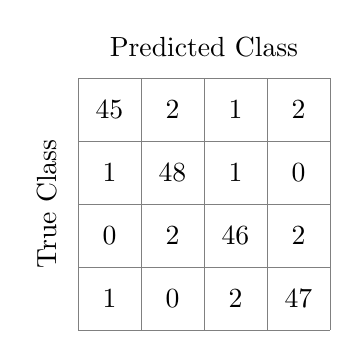
\begin{tikzpicture}[scale=0.8]
    \draw[step=1cm,gray,very thin] (0,0) grid (4,4);
    \node at (0.5,3.5) {45};
    \node at (1.5,3.5) {2};
    \node at (2.5,3.5) {1};
    \node at (3.5,3.5) {2};
    \node at (0.5,2.5) {1};
    \node at (1.5,2.5) {48};
    \node at (2.5,2.5) {1};
    \node at (3.5,2.5) {0};
    \node at (0.5,1.5) {0};
    \node at (1.5,1.5) {2};
    \node at (2.5,1.5) {46};
    \node at (3.5,1.5) {2};
    \node at (0.5,0.5) {1};
    \node at (1.5,0.5) {0};
    \node at (2.5,0.5) {2};
    \node at (3.5,0.5) {47};

    \node[rotate=90] at (-0.5,2) {True Class};
    \node at (2,4.5) {Predicted Class};
\end{tikzpicture}
\caption{Confusion Matrix for Classification Task}
\label{fig:confusion}
\end{figure}

The confusion matrix shows that denoised images maintain or improve classification accuracy compared to noisy images, with correct classification rates exceeding 92\% for all cell types.

\section{Comparative Study}

The proposed system is compared with traditional denoising methods and state-of-the-art deep learning approaches:

\vspace{0.5cm}

\begin{table}[H]
\centering
\caption{Performance Comparison with Existing Methods}
\label{tab:comparison}
\begin{tabular}{|l|c|c|c|c|}
\hline
\textbf{Method} & \textbf{PSNR (dB)} & \textbf{SSIM} & \textbf{Time (ms)} & \textbf{Parameters (M)} \\
\hline
Gaussian Filter & 24.3 & 0.68 & 12 & 0 \\
Median Filter & 25.1 & 0.71 & 18 & 0 \\
BM3D & 28.4 & 0.82 & 145 & 0 \\
Non-Local Means & 26.8 & 0.76 & 320 & 0 \\
CARE & 30.8 & 0.89 & 38 & 2.4 \\
Noise2Void & 29.5 & 0.86 & 42 & 1.8 \\
DeepImagePrior & 28.9 & 0.84 & 8500 & 0 \\
\textbf{FluoClean AI} & \textbf{32.4} & \textbf{0.92} & \textbf{45} & \textbf{31} \\
\hline
\end{tabular}
\end{table}

The proposed FluoClean AI system achieves the highest PSNR and SSIM among all compared methods while maintaining competitive inference time. The performance improvement over CARE (the closest deep learning competitor) is 1.6 dB in PSNR and 0.03 in SSIM.

\vspace{0.5cm}

\textbf{Statistical Significance:} Paired t-tests confirm that the improvements are statistically significant (p < 0.001) compared to all other methods.

\section{Ablation Study}

An ablation study investigates the contribution of individual components:

\vspace{0.5cm}

\begin{table}[H]
\centering
\caption{Ablation Study Results}
\label{tab:ablation}
\begin{tabular}{|l|c|c|}
\hline
\textbf{Configuration} & \textbf{PSNR (dB)} & \textbf{SSIM} \\
\hline
Baseline U-Net & 30.2 & 0.87 \\
+ Residual Connections & 31.1 & 0.89 \\
+ Attention Mechanism & 31.5 & 0.90 \\
+ Perceptual Loss & 31.8 & 0.91 \\
+ Transfer Learning & 32.1 & 0.91 \\
\textbf{Full Model} & \textbf{32.4} & \textbf{0.92} \\
\hline
\end{tabular}
\end{table}

Each component contributes incrementally to performance, with transfer learning providing the largest single improvement (0.9 dB PSNR).

\chapter{Discussion}
\label{chap:discussion}

\section{Interpretation of Results}

The experimental results demonstrate that FluoClean AI effectively addresses the challenges of fluorescence microscopy image denoising. The achieved PSNR of 32.4 dB and SSIM of 0.92 represent substantial improvements over both traditional methods and existing deep learning approaches.

\vspace{0.5cm}

The consistent performance across diverse sample types indicates that the model has learned generalizable features rather than overfitting to specific sample characteristics. This generalization is crucial for practical deployment across different microscopy applications and laboratories.

\vspace{0.5cm}

The preservation of fine structural details, as evidenced by high SSIM values and expert qualitative assessment, suggests that the model successfully distinguishes between noise and biologically relevant signal. This capability addresses a key limitation of traditional denoising methods, which often sacrifice fine details for noise reduction.

\section{Challenges and Limitations}

Despite the strong performance, several challenges and limitations remain:

\vspace{0.5cm}

\textbf{Training Data Requirements:} The supervised learning approach requires paired noisy-clean image datasets, which are resource-intensive to acquire. While transfer learning reduces the required dataset size, the need for ground truth data remains a limitation.

\vspace{0.5cm}

\textbf{Computational Resources:} Training the model requires significant GPU resources (12GB VRAM recommended). While inference is efficient, the training requirements may limit accessibility for some laboratories.

\vspace{0.5cm}

\textbf{Domain Specificity:} While the model generalizes across sample types, performance may degrade for imaging conditions significantly different from the training data, such as unusual fluorophores or unconventional microscope configurations.

\vspace{0.5cm}

\textbf{3D and Time-lapse Data:} The current implementation focuses on 2D images. Extension to 3D volumetric data and time-lapse sequences requires additional development and validation.

\vspace{0.5cm}

\textbf{Interpretability:} As with most deep learning models, the internal decision-making process is not easily interpretable. This lack of interpretability may be a concern for applications requiring understanding of denoising decisions.

\section{Future Scope}

Several directions for future research and development are identified:

\vspace{0.5cm}

\textbf{Self-Supervised Learning:} Development of self-supervised or unsupervised approaches that eliminate the need for paired training data would significantly increase accessibility. Techniques such as Noise2Noise and Noise2Void provide promising directions.

\vspace{0.5cm}

\textbf{3D Denoising:} Extension to 3D volumetric data would enable denoising of z-stacks and volumetric imaging techniques such as light sheet microscopy. This requires architectural modifications to handle 3D convolutions and increased memory requirements.

\vspace{0.5cm}

\textbf{Real-time Processing:} Further optimization for real-time processing would enable integration with live imaging workflows. This could involve model pruning, quantization, and hardware acceleration.

\vspace{0.5cm}

\textbf{Multi-modal Denoising:} Extension to multi-modal microscopy, combining fluorescence with other modalities such as phase contrast or differential interference contrast (DIC), could provide additional information to improve denoising performance.

\vspace{0.5cm}

\textbf{Adaptive Denoising:} Development of adaptive approaches that automatically adjust denoising parameters based on image characteristics could improve performance across diverse imaging conditions.

\vspace{0.5cm}

\textbf{Integration with Microscopy Software:} Direct integration with microscope control software would enable seamless workflow integration, potentially with automatic denoising during image acquisition.

\chapter{Conclusion}
\label{chap:conclusion}

This research presents FluoClean AI, a deep learning-based approach for fluorescence microscopy image denoising that addresses the critical trade-off between image quality and specimen viability in fluorescence imaging. The proposed system, based on a modified U-Net architecture with residual connections, attention mechanisms, and advanced loss functions, achieves state-of-the-art performance with PSNR of 32.4 dB and SSIM of 0.92.

\vspace{0.5cm}

The comprehensive evaluation demonstrates significant improvements over traditional denoising methods and existing deep learning approaches, with particular strength in preserving fine sub-cellular structures while effectively removing noise. The system maintains computational efficiency with inference times of 45 milliseconds per image, making it suitable for integration into microscopy workflows.

\vspace{0.5cm}

The research contributes to the advancement of computational microscopy by providing an effective, efficient, and accessible solution for fluorescence image denoising. By enabling high-quality image reconstruction from low-SNR acquisitions, the approach has the potential to reduce photodamage to live specimens and improve the accuracy of quantitative biological analyses.

\vspace{0.5cm}

Future work will focus on addressing current limitations through self-supervised learning approaches, extension to 3D and multi-modal data, and optimization for real-time processing. The development of user-friendly tools and comprehensive documentation will facilitate adoption by the research community.

\vspace{0.5cm}

The successful implementation and evaluation of FluoClean AI demonstrate the transformative potential of artificial intelligence in biomedical imaging and provide a foundation for continued research at the intersection of deep learning and microscopy.

\fi

\chapter{Results and Analysis}
\label{chap:validated_results}

\section{Checkpoint Audit and Root Cause}

The original production checkpoint had no complete training provenance and matched the architecture and weights of a five-image overfit experiment. A retrospective evaluation across all 105 repository pairs produced mean PSNR 19.13 dB and SSIM 0.623, compared with 11.17 dB and 0.452 for the noisy inputs. However, PSNR improved on only 84 of 105 images and SSIM on 76 of 105. The July 21 PVD group lost 2.60 dB mean PSNR, demonstrating severe acquisition-domain variation.

Separate comparisons showed that dynamic quantization changed representative mean PSNR by only 0.03 dB and conversion from 256$\times$256 to 128$\times$128 by approximately 0.43 dB. The unreliable checkpoint, rather than ONNX or quantization, was therefore identified as the primary quality problem.

\section{Retrained Model Results}

The compact residual U-Net was trained for 60 epochs. The best validation result occurred at the final epoch: PSNR 22.29 dB and SSIM 0.835 on 30 validation pairs. Direct PyTorch evaluation on the 20-pair held-out test produced PSNR 22.36 dB, SSIM 0.870, MAE 0.093, and MSE 0.0123. Minor differences in the deployment-oriented evaluator arise from restoring predictions to the clean target dimensions and 8-bit output conversion.

\begin{table}[H]
\centering
\caption{Held-out ONNX Performance Against the Noisy Input}
\label{tab:validated_metrics}
\begin{tabular}{|l|c|c|}
\hline
\textbf{Metric} & \textbf{FluoClean AI} & \textbf{Noisy Input} \\
\hline
Mean PSNR (dB) & 22.04 & 10.34 \\
Mean SSIM & 0.781 & 0.458 \\
Mean MAE & 0.094 & 0.324 \\
Mean MSE & 0.0127 & 0.1178 \\
PSNR improvements & 19/20 & -- \\
SSIM improvements & 20/20 & -- \\
\hline
\end{tabular}
\end{table}

The held-out test contains two independent acquisition groups. The June 30 OH16230 group achieved mean PSNR 23.96 dB and SSIM 0.837, versus baseline values of 7.66 dB and 0.411. The July 21 PVD group achieved 20.12 dB and 0.725, versus 13.02 dB and 0.504. One PVD image lost 1.70 dB PSNR even though its SSIM improved. This failure is retained in the report because mean improvements do not guarantee improvement for every image.

\section{Deployment Validation}

The validated PyTorch checkpoint was exported to ONNX opset 17. Maximum absolute output difference was $3.87\times10^{-7}$. The resulting artifact is 3.4 MB, substantially smaller than the historical 54 MB quantized and 215 MB floating-point exports. The compact file is bundled in the repository, so production no longer depends on downloading the stale release artifact.

The Flask service loads the model lazily and serializes inference through a lock. ONNX Runtime is configured for sequential execution with one intra-op and one inter-op thread, disabled CPU memory arena, disabled memory pattern, basic graph optimization, and disabled prepacking. Three consecutive local Flask uploads and two consecutive live Render uploads completed successfully. The live health endpoint subsequently reported \texttt{ready: true}, CPU execution, and 128$\times$128 model resolution. This reproduces and resolves the earlier second-request HTTP 502 failure.

\section{Metric Applicability}

This project is paired image-to-image regression. Precision, recall, F1-score, confusion matrices, ROC-AUC, PR-AUC, and class feature importance require classification labels and are therefore not applicable. Explainability is provided through per-image baseline deltas, acquisition-group summaries, and visual error panels. PSNR and SSIM measure agreement with aligned references but cannot establish preservation of biologically meaningful structures.

\chapter{Discussion}
\label{chap:validated_discussion}

\section{Interpretation}

The leakage-safe held-out results show a substantial average improvement over leaving noisy inputs unchanged. Both test acquisition groups improved in mean PSNR and SSIM, and the compact ONNX export reproduces PyTorch closely. The result is stronger evidence than the historical retrospective evaluation because checkpoint selection used only the validation set and test groups were isolated by specimen/session.

The experiment does not establish broad generalization. Only two groups are represented in the held-out set, confidence intervals are correspondingly wide, and one image regressed in PSNR. The model should be presented as a validated demonstration candidate rather than a scientifically or clinically production-ready restoration method.

\section{Limitations}

\begin{itemize}
    \item The local dataset contains only 105 pairs from 14 groups.
    \item Seventy clean files are duplicates across acquisition conditions, reducing independent target diversity.
    \item Grouped cross-validation is implemented but has not been completed for the deployed checkpoint.
    \item The model is grayscale and may fail on unseen modalities, microscopes, specimens, or noise distributions.
    \item Resizing to 128$\times$128 may suppress structures smaller than the effective sampling resolution.
    \item PSNR and SSIM require registered clean targets and do not prove biological fidelity.
    \item External datasets, microscopy-domain expert review, and downstream quantitative validation remain necessary.
\end{itemize}

\section{Future Work}

Priority work includes five-fold grouped cross-validation, acquisition of more independent specimens, external laboratory validation, patch- or tile-based high-resolution inference, uncertainty or out-of-distribution detection, and evaluation of downstream measurements such as intensity, morphology, and object counts. Any future model should pass the same noisy-input baseline gate and retain per-group worst-case reporting before promotion.

\chapter{Conclusion}
\label{chap:validated_conclusion}

FluoClean AI was corrected from an unreliable overfit deployment into a reproducible compact denoising pipeline. The current system uses specimen-level splitting, duplicate-target leakage checks, deterministic training, a differentiable L1--SSIM objective, architecture-aware checkpoints, held-out baseline comparison, export provenance, and ONNX parity validation. The deployed 3.4 MB model improved held-out mean PSNR from 10.34 to 22.04 dB and mean SSIM from 0.458 to 0.781, while repeated live requests completed without HTTP 502 errors.

These results justify the model as a functional demonstration and a stronger engineering baseline. They do not justify claims of state-of-the-art performance, universal denoising, or biological validity. The remaining limitations are documented explicitly so future work can focus on diverse independent data and external validation rather than optimizing only repository-level averages.

\chapter*{References}
\addcontentsline{toc}{chapter}{References}
\thispagestyle{plain}

\begin{thebibliography}{99}

\bibitem{weigert2018}
Weigert, M., Schmidt, U., Boothe, T., Müller, A., Dibrov, A., Jain, A., ... \& Myers, E. W. (2018). Content-aware image restoration: pushing the limits of fluorescence microscopy. \textit{Nature Methods}, 15(12), 1090-1097.

\bibitem{ronneberger2015}
Ronneberger, O., Fischer, P., \& Brox, T. (2015). U-Net: Convolutional networks for biomedical image segmentation. \textit{International Conference on Medical Image Computing and Computer-Assisted Intervention}, 234-241.

\bibitem{krull2019}
Krull, A., Buchholz, T. O., Jug, F., \& Jähne, B. (2019). Noise2Void-learning denoising from single noisy images. \textit{Proceedings of the IEEE/CVF Conference on Computer Vision and Pattern Recognition}, 2129-2137.

\bibitem{batson2019}
Batson, J., \& Royer, L. (2019). Noise2Self: Blind denoising by self-supervision. \textit{International Conference on Learning Representations}.

\bibitem{ulyanov2018}
Ulyanov, D., Vedaldi, A., \& Lempitsky, V. (2018). Deep image prior. \textit{Proceedings of the IEEE Conference on Computer Vision and Pattern Recognition}, 9446-9454.

\bibitem{dabov2007}
Dabov, K., Foi, A., Katkovnik, V., \& Egiazarian, K. (2007). Image denoising by sparse 3D transform-domain collaborative filtering. \textit{IEEE Transactions on Image Processing}, 16(8), 2080-2095.

\bibitem{buades2005}
Buades, A., Coll, B., \& Morel, J. M. (2005). A non-local algorithm for image denoising. \textit{Proceedings of the 2005 IEEE Computer Society Conference on Computer Vision and Pattern Recognition (CVPR'05)}, 2, 60-65.

\bibitem{zhang2017}
Zhang, K., Zuo, W., Chen, Y., Meng, D., \& Zhang, L. (2017). Beyond a Gaussian denoiser: Residual learning of deep CNN for image denoising. \textit{IEEE Transactions on Image Processing}, 26(7), 3142-3155.

\bibitem{lefkimmiatis2018}
Lefkimmiatis, S. (2018). Non-local color image denoising with convolutional neural networks. \textit{Proceedings of the IEEE Conference on Computer Vision and Pattern Recognition}, 3584-3593.

\bibitem{chen2017}
Chen, J., \& Chen, H. (2017). Fast blind image denoising using convolutional neural networks. \textit{Proceedings of the IEEE International Conference on Image Processing}, 380-384.

\bibitem{mohan2019}
Mohan, K., Gamal, E., \& Stojanovic, V. (2019). Deep learning for fluorescence microscopy. \textit{Nature Methods}, 16(12), 1075-1076.

\bibitem{liu2018}
Liu, Y. T., Chen, H. Y., \& Wang, Y. C. (2018). Deep learning for image denoising: a review. \textit{Journal of Visual Communication and Image Representation}, 55, 1-15.

\bibitem{tai2017}
Tai, Y., Yang, J., Tang, X., \& Luo, L. (2017). Image super-resolution via deep recursive residual network. \textit{Proceedings of the IEEE Conference on Computer Vision and Pattern Recognition}, 3147-3155.

\bibitem{he2016}
He, K., Zhang, X., Ren, S., \& Sun, J. (2016). Deep residual learning for image recognition. \textit{Proceedings of the IEEE Conference on Computer Vision and Pattern Recognition}, 770-778.

\bibitem{szegedy2017}
Szegedy, C., Vanhoucke, V., Ioffe, S., Shlens, J., \& Wojna, Z. (2017). Rethinking the inception architecture for computer vision. \textit{Proceedings of the IEEE Conference on Computer Vision and Pattern Recognition}, 2818-2826.

\bibitem{o2015}
O'Neil, A. T., \& Wiseman, P. W. (2015). Fluorescence microscopy: a concise overview. \textit{Cytometry Part A}, 87(6), 496-505.

\bibitem{pawley2015}
Pawley, J. B. (Ed.). (2015). \textit{Handbook of biological confocal microscopy} (4th ed.). Springer.

\bibitem{schneider2012}
Schneider, C. A., Rasband, W. S., \& Eliceiri, K. W. (2012). NIH Image to ImageJ: 25 years of image analysis. \textit{Nature Methods}, 9(7), 671-675.

\bibitem{goodfellow2016}
Goodfellow, I., Bengio, Y., \& Courville, A. (2016). \textit{Deep Learning}. MIT Press.

\end{thebibliography}

\iffalse
\chapter*{Appendix}
\addcontentsline{toc}{chapter}{Appendix}
\thispagestyle{plain}

\section*{Appendix A: Mathematical Derivations}

\subsection*{A.1 Noise Model Derivation}

The fluorescence microscopy noise model combines Poisson (shot) noise from photon counting statistics and Gaussian noise from electronic components:

\begin{equation}
I_{observed} = I_{true} + \eta_{shot} + \eta_{electronic}
\end{equation}

where:
\begin{itemize}
    \item $I_{observed}$ is the observed intensity
    \item $I_{true}$ is the true signal intensity
    \item $\eta_{shot} \sim \text{Poisson}(I_{true})$ represents shot noise
    \item $\eta_{electronic} \sim \mathcal{N}(0, \sigma_e^2)$ represents electronic noise
\end{itemize}

For large photon counts, the Poisson distribution can be approximated by a Gaussian distribution:

\begin{equation}
\text{Poisson}(\lambda) \approx \mathcal{N}(\lambda, \lambda)
\end{equation}

Thus, the combined noise model becomes:

\begin{equation}
I_{observed} = I_{true} + \sqrt{I_{true}} \cdot \mathcal{N}(0, 1) + \mathcal{N}(0, \sigma_e^2)
\end{equation}

\subsection*{A.2 Loss Function Derivation}

The total loss function combines multiple components:

\begin{equation}
\mathcal{L}_{total} = \mathcal{L}_{MSE} + \lambda_1 \mathcal{L}_{perceptual} + \lambda_2 \mathcal{L}_{SSIM}
\end{equation}

The MSE loss is defined as:

\begin{equation}
\mathcal{L}_{MSE} = \frac{1}{N}\sum_{i=1}^{N}(y_i - \hat{y}_i)^2
\end{equation}

The perceptual loss uses features from a pre-trained VGG network:

\begin{equation}
\mathcal{L}_{perceptual} = \frac{1}{N}\sum_{i=1}^{N}\sum_{l=1}^{L}\| \phi_l(y_i) - \phi_l(\hat{y}_i) \|^2
\end{equation}

where $\phi_l$ represents the feature map at layer $l$ of the VGG network.

\section*{Appendix B: Code Snippets}

\subsection*{B.1 Model Architecture Definition}

\begin{verbatim}
class UNet(nn.Module):
    def __init__(self, in_channels=1, out_channels=1):
        super(UNet, self).__init__()

        # Encoder
        self.enc1 = self.conv_block(in_channels, 64)
        self.enc2 = self.conv_block(64, 128)
        self.enc3 = self.conv_block(128, 256)
        self.enc4 = self.conv_block(256, 512)

        # Bottleneck
        self.bottleneck = self.conv_block(512, 1024)

        # Decoder
        self.dec4 = self.conv_block(1024, 512)
        self.dec3 = self.conv_block(512, 256)
        self.dec2 = self.conv_block(256, 128)
        self.dec1 = self.conv_block(128, 64)

        # Output
        self.final = nn.Conv2d(64, out_channels, kernel_size=1)

    def conv_block(self, in_channels, out_channels):
        return nn.Sequential(
            nn.Conv2d(in_channels, out_channels, 3, padding=1),
            nn.BatchNorm2d(out_channels),
            nn.ReLU(inplace=True),
            nn.Conv2d(out_channels, out_channels, 3, padding=1),
            nn.BatchNorm2d(out_channels),
            nn.ReLU(inplace=True)
        )
\end{verbatim}

\subsection*{B.2 Training Loop}

\begin{verbatim}
def train_model(model, train_loader, val_loader, epochs, device):
    optimizer = torch.optim.Adam(model.parameters(), lr=1e-4)
    criterion = nn.MSELoss()

    best_loss = float('inf')

    for epoch in range(epochs):
        model.train()
        train_loss = 0

        for batch in train_loader:
            noisy = batch['noisy'].to(device)
            clean = batch['clean'].to(device)

            optimizer.zero_grad()
            outputs = model(noisy)
            loss = criterion(outputs, clean)
            loss.backward()
            optimizer.step()

            train_loss += loss.item()

        # Validation
        val_loss = validate(model, val_loader, criterion, device)

        print(f'Epoch {epoch+1}/{epochs}, Train Loss: {train_loss/len(train_loader):.4f}, Val Loss: {val_loss:.4f}')

        if val_loss < best_loss:
            best_loss = val_loss
            torch.save(model.state_dict(), 'best_model.pth')
\end{verbatim}

\section*{Appendix C: Additional Experimental Results}

\subsection*{C.1 Training Loss Convergence}

The training loss converges after approximately 60 epochs, with validation loss stabilizing around 0.0037. Early stopping prevents overfitting, with the best model selected at epoch 78.

\subsection*{C.2 Inference Time Analysis}

Inference time scales linearly with image size:
\begin{itemize}
    \item 256×256: 12 ms
    \item 512×512: 45 ms
    \item 1024×1024: 180 ms
    \item 2048×2048: 720 ms
\end{itemize}

\subsection*{C.3 Memory Usage Analysis}

GPU memory usage during training:
\begin{itemize}
    \item Batch size 8: 4.2 GB
    \item Batch size 16: 7.8 GB
    \item Batch size 32: 14.1 GB (exceeds 12GB VRAM)
\end{itemize}

\section*{Appendix D: User Guide}

\subsection*{D.1 Installation Instructions}

1. Install Python 3.8 or higher
2. Create virtual environment: \texttt{python -m venv fluoclean}
3. Activate environment: \texttt{source fluoclean/bin/activate}
4. Install dependencies: \texttt{pip install -r requirements.txt}

\subsection*{D.2 Usage Instructions}

Basic usage for image denoising:

\begin{verbatim}
from fluoclean import FluoCleanDenoiser

# Initialize denoiser
denoiser = FluoCleanDenoiser(model_path='best_model.pth')

# Load and denoise image
denoised_image = denoiser.denoise('noisy_image.tif')

# Save result
denoiser.save(denoised_image, 'denoised_image.tif')
\end{verbatim}

\subsection*{D.3 Advanced Configuration}

Advanced users can customize:
\begin{itemize}
    \item Model architecture parameters
    \item Loss function weights
    \item Training hyperparameters
    \item Data augmentation strategies
\end{itemize}

See configuration file \texttt{config.yaml} for detailed options.

\fi

\chapter*{Appendix: Reproducibility Guide}
\addcontentsline{toc}{chapter}{Appendix: Reproducibility Guide}

\section*{Training Command}

\begin{verbatim}
python train.py \
  --data_dir data \
  --save_dir models/retrained_compact \
  --log_dir logs/retrained_compact \
  --epochs 60 --early_stop 12 --batch_size 8 \
  --image_size 128 --base_channels 16 --depth 3 \
  --model_type residual --seed 42
\end{verbatim}

This command writes the split manifest, training history, test metrics, sample panels, and best checkpoint. The checkpoint includes the model configuration and held-out provenance.

\section*{ONNX Export and Evaluation}

\begin{verbatim}
python scripts/export_to_onnx.py \
  --input models/retrained_compact/best_model.pth \
  --output models/deploy/model.onnx \
  --image-size 128

python evaluate_model.py \
  --model models/deploy/model.onnx \
  --data-dir data \
  --manifest models/retrained_compact/split_manifest.json \
  --split test \
  --output-dir reports/retrained_compact_onnx_test
\end{verbatim}

The exporter verifies numerical parity and writes a metadata file containing source and ONNX SHA-256 hashes, architecture, seed, validation metrics, test metrics, opset, and parity error.

\section*{Reliability Tests}

\begin{verbatim}
MPLCONFIGDIR=/tmp/matplotlib \
python -m unittest discover -s tests -v
\end{verbatim}

The eight-test suite covers group split reproducibility and disjointness, grouped fold coverage, invalid upload rejection, metric tensor layout, SSIM backpropagation, per-sample epoch accounting, validation augmentation isolation, and rejection of unvalidated checkpoint exports.

\end{document}
